%% ============================================================
%%  20-Minute Defense: Hybrid Spectral-Matching + Deep Learning
%%  Raman Mineral Identification System
%%  Rahul [Surname]  |  May 8, 2026
%% ============================================================
\documentclass[aspectratio=169,10pt]{beamer}

%% ─── Packages ────────────────────────────────────────────────
\usepackage[T1]{fontenc}
\usepackage[utf8]{inputenc}
\usepackage{lmodern}
\usepackage{amsmath,amssymb,mathtools}
\usepackage{bm}
\usepackage{booktabs}
\usepackage{array}
\usepackage{colortbl}
\usepackage{xcolor}
\usepackage{tikz}
\usetikzlibrary{arrows.meta,shapes.geometric,positioning,calc}
\usepackage{tcolorbox}
\tcbuselibrary{skins,breakable}
\usepackage{algorithm}
\usepackage{algpseudocode}
\usepackage{microtype}
\usepackage{ragged2e}

%% ─── Colours ─────────────────────────────────────────────────
\definecolor{headerbg}{RGB}{28,58,94}
\definecolor{accent}{RGB}{139,26,26}
\definecolor{mathbg}{RGB}{238,244,250}
\definecolor{accentbg}{RGB}{245,230,232}
\definecolor{greenbg}{RGB}{232,248,232}
\definecolor{yellowbg}{RGB}{255,248,215}
\definecolor{tealblue}{RGB}{58,124,165}
\definecolor{darktext}{RGB}{26,26,26}
\definecolor{lightblue}{RGB}{168,200,232}

%% ─── Beamer theme ────────────────────────────────────────────
\usetheme{default}
\usecolortheme{default}

\setbeamercolor{frametitle}{fg=white,bg=headerbg}
\setbeamercolor{normal text}{fg=darktext,bg=white}
\setbeamercolor{structure}{fg=headerbg}
\setbeamercolor{itemize item}{fg=headerbg}
\setbeamercolor{itemize subitem}{fg=tealblue}
\setbeamercolor{enumerate item}{fg=headerbg}
\setbeamercolor{enumerate subitem}{fg=tealblue}
\setbeamercolor{alerted text}{fg=accent}
\setbeamercolor{block title}{fg=white,bg=headerbg}
\setbeamercolor{block body}{fg=darktext,bg=mathbg}

\setbeamerfont{frametitle}{series=\bfseries,size=\large}
\setbeamerfont{title}{series=\bfseries,size=\Large}
\setbeamerfont{block title}{series=\bfseries,size=\small}

%% Navigation off
\setbeamertemplate{navigation symbols}{}

%% Frame title: full-width dark bar + left crimson rule
\setbeamertemplate{frametitle}{%
  \nointerlineskip%
  \begin{beamercolorbox}[%
      wd=\paperwidth,ht=0.62cm,dp=0.10cm,leftskip=0pt]{frametitle}%
    \textcolor{accent}{\vrule width 0.07cm height 0.72cm depth 0pt}%
    \hspace{0.12cm}%
    \usebeamerfont{frametitle}\insertframetitle%
  \end{beamercolorbox}%
}

%% Footer: page number only, bottom-right
\setbeamertemplate{footline}{%
  \hfill%
  \textcolor{gray!80}{\scriptsize\insertframenumber/\inserttotalframenumber}%
  \hspace*{0.22cm}\vspace*{0.10cm}%
}

%% Itemize bullets
\setbeamertemplate{itemize item}{\small$\blacktriangleright$}
\setbeamertemplate{itemize subitem}{\small$\triangleright$}

%% ─── tcolorbox styles ────────────────────────────────────────
\tcbset{
  mathbox/.style={
    enhanced, colback=mathbg, colframe=tealblue!55,
    boxrule=0.55pt, arc=2pt,
    left=6pt, right=6pt, top=4pt, bottom=4pt
  },
  insightbox/.style={
    enhanced, colback=yellowbg, colframe=orange!55!brown,
    borderline west={2.5pt}{0pt}{orange!65!brown},
    boxrule=0.35pt, arc=0pt,
    left=8pt, right=6pt, top=3pt, bottom=3pt
  },
  whybox/.style={
    enhanced, colback=greenbg, colframe=green!50!black,
    borderline west={2.5pt}{0pt}{green!55!black},
    boxrule=0.35pt, arc=0pt,
    left=8pt, right=6pt, top=3pt, bottom=3pt
  },
  notebox/.style={
    enhanced, colback=yellowbg, colframe=orange!55!brown,
    borderline west={2.5pt}{0pt}{orange!65!brown},
    boxrule=0.35pt, arc=0pt,
    left=8pt, right=6pt, top=3pt, bottom=3pt
  },
  domainbox/.style={
    enhanced, colback=mathbg!70, colframe=tealblue!40,
    title style={colback=headerbg},
    fonttitle=\color{white}\bfseries\footnotesize,
    arc=2pt, boxrule=0.5pt,
    attach boxed title to top left={yshift=-2mm, xshift=4mm},
    left=6pt, right=6pt, top=10pt, bottom=4pt
  },
}

%% ─── Math shorthands ─────────────────────────────────────────
\newcommand{\qt}{\tilde{\mathbf{q}}}
\newcommand{\calL}{\mathcal{L}}
\newcommand{\calR}{\mathcal{R}}
\newcommand{\norm}[1]{\left\|#1\right\|}
\DeclareMathOperator*{\argmax}{arg\,max}
\DeclareMathOperator*{\argmin}{arg\,min}

%% ─── Metadata ────────────────────────────────────────────────
\title{A Hybrid Spectral-Matching and Deep-Learning System\\[2pt]
       for Real-Time Mineral Identification from Raman Spectra}
\subtitle{Final Project Defense \textemdash{} 20-Minute Version}
\author{Rahul Athipatla\\[0.25em]
        {\small Under the supervision of Rousan Debbarma \& Aparna Mehra}}
\date{May~8,~2026\\[0.15em]
      {\scriptsize Department of Mathematics\enspace$\cdot$\enspace IIT Delhi}}

%% =============================================================
\begin{document}
%% =============================================================

%% ── SLIDE 1: Title ──────────────────────────────────────────
{%
\setbeamercolor{background canvas}{bg=headerbg}
\setbeamertemplate{footline}{}%
\begin{frame}[plain]
  \vspace{0.45cm}
  \textcolor{accent}{\rule{\linewidth}{0.07cm}}\par
  \vspace{0.28cm}
  {%
    \usebeamerfont{title}\color{white}
    \inserttitle\par
  }
  \vspace{0.18cm}
  \textcolor{tealblue!70}{\rule{\linewidth}{0.03cm}}\par
  \vspace{0.18cm}
  {\small\color{white!80}\insertsubtitle}\par
  \vspace{0.28cm}
  {\normalsize\bfseries\color{white}\insertauthor}\par
  \vspace{0.12cm}
  {\small\color{white!75}\insertdate}\par
  \vspace{0.38cm}
  \textcolor{accent}{\rule{\linewidth}{0.07cm}}
\end{frame}
}%

%% ── SLIDE 2: Problem & Motivation ──────────────────────────
\begin{frame}{The Mineral-Identification Problem}
  \begin{columns}[T]
    \begin{column}{0.62\textwidth}
      Raman scattering produces a vibrational spectrum
      $\{(\nu_i,I_i)\}_{i=1}^N$ acting as a mineral fingerprint:\par
      \vspace{0.2cm}
      \begin{tcolorbox}[mathbox]
        \[
          I(\nu)=\sum_k A_k\,\mathcal{L}(\nu;\nu_k,\gamma_k)+B(\nu)+\eta(\nu)
        \]
        \centering\footnotesize
        $\mathcal{L}$ = Lorentzian profile\quad
        $B(\nu)$ = fluorescence baseline\quad
        $\eta$ = detector noise
      \end{tcolorbox}
      \vspace{0.18cm}
      {\small\bfseries\color{headerbg}Why automate identification?}
      \begin{itemize}\setlength\itemsep{0.10cm}\small
        \item Field instruments now exist; expert peak-matching does not scale.
        \item RRUFF covers $>4\,000$ species --- manual lookup is the dominant bottleneck.
        \item Task: estimate $\{(\nu_k,A_k,\gamma_k)\}$ from $I(\nu)$ and match
              a reference library.
      \end{itemize}
    \end{column}
    \begin{column}{0.35\textwidth}
      \begin{tcolorbox}[domainbox, title={Domains directly affected}]
        \footnotesize
        \begin{itemize}\setlength\itemsep{0.10cm}
          \item Geology \& planetary science\\(Mars SHERLOC)
          \item Cultural-heritage pigment analysis
          \item Forensic mineralogy
          \item Mining process monitoring
        \end{itemize}
      \end{tcolorbox}
    \end{column}
  \end{columns}
\end{frame}

%% ── SLIDE 3: Formal Problem Statement ──────────────────────
\begin{frame}{Formal Problem Statement}
  \textbf{\color{accent}Given}\enspace
  unknown query $\mathbf{q}=\{(\nu_i,I_i)\}_{i=1}^N$ and reference
  library $\mathcal{R}=\{\mathbf{r}_m\}_{m=1}^M$ on canonical grid
  $\boldsymbol{\nu}_*\in\mathbb{R}^P$.

  \vspace{0.12cm}
  \textbf{\color{accent}Produce}
  \begin{enumerate}\setlength\itemsep{0.08cm}\small
    \item Ranked list $\bigl((m_1,c_1),\ldots,(m_K,c_K)\bigr)$,\quad
          confidences $c_{(k)}\in[0,1]$.
    \item Non-negative weight vector
          $\mathbf{x}\in\mathbb{R}^M_{\ge0}$ such that
          $\norm{A^\top\mathbf{x}-\tilde{\mathbf{q}}}_2$ is minimised,
          where $A$ is the row-stacked reference matrix and $\tilde{\mathbf{q}}$
          the preprocessed query.
  \end{enumerate}

  \smallskip
  \textbf{\color{accent}Subject to}\enspace
  wall-clock budget $\tau\le 1\,\text{s}$ on a laptop GPU (16\,GB RAM).

  \vspace{0.18cm}
  {\small\bfseries\color{headerbg}Key design choices}

  \smallskip
  \footnotesize
  \begin{tabular}{@{}llp{4.6cm}@{}}
    \toprule
    \textbf{Parameter} & \textbf{Value adopted} & \textbf{Consequence}\\
    \midrule
    Canonical grid & $[100,4000]\,\text{cm}^{-1}$, $\Delta\nu=2\,\text{cm}^{-1}$
                   & $P=1\,951$ channels\\[1pt]
    Library size $M$ & $2\,481$ unique minerals
                     & Synthetic-25 $\cup$ RRUFF-2456\\[1pt]
    Top-$K$          & $K=5$  & Aligns with expert workflow\\[1pt]
    Peak model       & Lorentzian & Matches optical-phonon lifetime broadening\\
    \bottomrule
  \end{tabular}
\end{frame}

%% ── SLIDE 4: System Architecture ───────────────────────────
\begin{frame}{End-to-End System Architecture}
  \vspace{-0.1cm}
  \begin{center}
  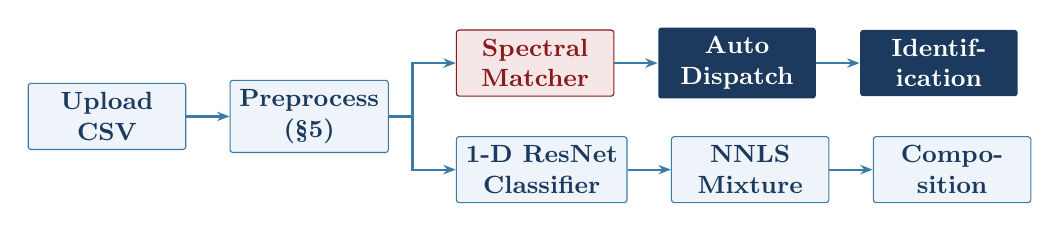
\begin{tikzpicture}[
    box/.style    = {rectangle, draw=tealblue,  fill=mathbg,   minimum width=2.0cm,
                     minimum height=0.72cm, align=center,
                     font=\small\bfseries\color{headerbg}, rounded corners=1pt},
    darkbox/.style= {rectangle, fill=headerbg,                 minimum width=2.0cm,
                     minimum height=0.72cm, align=center,
                     font=\small\bfseries\color{white}, rounded corners=1pt},
    redbox/.style = {rectangle, draw=accent, fill=accentbg,   minimum width=2.0cm,
                     minimum height=0.72cm, align=center,
                     font=\small\bfseries\color{accent}, rounded corners=1pt},
    arr/.style    = {-{Stealth[length=4.5pt]}, thick, draw=tealblue},
    node distance = 0.5cm
  ]
    \node[box]     (csv) {Upload\\CSV};
    \node[box, right=0.55cm of csv] (pre) {Preprocess\\(\S5)};

    \coordinate (fork) at ($(pre.east)+(0.3cm,0)$);
    \node[redbox,  above right=0.25cm and 0.55cm of fork] (mat) {Spectral\\Matcher};
    \node[box,     below right=0.25cm and 0.55cm of fork] (cnn) {1-D ResNet\\Classifier};

    \node[darkbox, right=0.55cm of mat] (disp) {Auto\\Dispatch};
    \node[box,     right=0.55cm of cnn] (nnls) {NNLS\\Mixture};

    \node[darkbox, right=0.55cm of disp] (ident) {Identif-\\ication};
    \node[box,     right=0.55cm of nnls] (comp)  {Compo-\\sition};

    \draw[arr] (csv)  -- (pre);
    \draw[arr] (pre.east) -- ++(0.3,0) |- (mat.west);
    \draw[arr] (pre.east) -- ++(0.3,0) |- (cnn.west);
    \draw[arr] (mat)  -- (disp);
    \draw[arr] (cnn)  -- (nnls);
    \draw[arr] (disp) -- (ident);
    \draw[arr] (nnls) -- (comp);
  \end{tikzpicture}
  \end{center}

  \vspace{0.20cm}
  \begin{tcolorbox}[notebox, top=2pt, bottom=2pt]
    \small Spectral matching \emph{always} runs as a deterministic safety net.
    The classifier enters dispatch only if its top-1 confidence
    exceeds $\tau_{\min}=0.55$, preventing confidently-wrong
    out-of-distribution predictions.
  \end{tcolorbox}
\end{frame}

%% ── SLIDE 5: Preprocessing Pipeline ────────────────────────
\begin{frame}{Preprocessing Pipeline}
  Given raw $(\boldsymbol{\nu}_\text{raw},\mathbf{I}_\text{raw})$,
  produce $\tilde{\mathbf{q}}\in\mathbb{R}^P$ on the canonical grid:

  \vspace{0.12cm}
  \small
  \begin{enumerate}\setlength\itemsep{0.14cm}
    \item \textbf{Linear interpolation onto $\boldsymbol{\nu}_*$:}\quad
          $\mathbf{I}_\text{grid}=\mathrm{interp}(\boldsymbol{\nu}_*,
          \boldsymbol{\nu}_\text{raw},\mathbf{I}_\text{raw})$

    \item \textbf{Cosmic-ray suppression} (5-point neighbour-ratio test):\quad
          $I_i\;\mapsto\;\bar{I}_\text{nbr}
          \cdot\mathbf{1}\!\left[\dfrac{I_i}{\max_j I_j}>\rho\right]$

    \item \textbf{Savitzky--Golay smoothing:}\quad
          window $w=5$,\; polynomial order $p=3$

    \item \textbf{ALS baseline removal:}\quad
          $\displaystyle\min_{\mathbf{z}}\sum_i w_i(y_i-z_i)^2
          +\lambda\sum_i(\Delta^2 z_i)^2,
          \quad\lambda=10^5,\;p_\text{asym}=0.01$

    \item \textbf{Non-negative clip $+$ $\ell_2$ normalisation:}\quad
          $\tilde{\mathbf{q}}=\mathbf{z}/\norm{\mathbf{z}}_2$
  \end{enumerate}

  \vspace{0.18cm}
  \begin{tcolorbox}[insightbox]
    \small\textbf{Key insight: interpolation must precede smoothing.}
    Smoothing on the raw grid couples the SG window to the spectrometer's
    native step $\delta\nu$:\; $w_\text{phys}=w\cdot\delta\nu$.
    A CSV at $\delta\nu=4\,\text{cm}^{-1}$ with $w=11$ gives a
    $44\,\text{cm}^{-1}$ window --- wider than typical Raman FWHM.
    \textbf{Fix lifted Quartz top-1 from 41\,\% to 86\,\%.}
  \end{tcolorbox}
\end{frame}

%% ── SLIDE 6: Combined-Metric Spectral Matcher ───────────────
\begin{frame}{Combined-Metric Spectral Matcher}
  \begin{columns}[T]
    \begin{column}{0.54\textwidth}
      For preprocessed query $\tilde{\mathbf{q}}$ and reference row $\mathbf{r}_m$:
      \begin{tcolorbox}[mathbox, top=3pt, bottom=3pt]
        \[
          s(\tilde{\mathbf{q}},\mathbf{r}_m)
          =
          \underbrace{\tfrac{1}{2}\,\langle\tilde{\mathbf{q}},\,\hat{\mathbf{r}}_m\rangle}_{\text{cosine}}
          +
          \underbrace{\tfrac{1}{2}\,
            \bigl\langle\widehat{D^2\tilde{\mathbf{q}}},\;
                        \widehat{D^2\mathbf{r}_m}\bigr\rangle}_{D^2\text{-Pearson}}
        \]
        \centering\scriptsize
        $\hat{\mathbf{v}}=(\mathbf{v}-\bar{v}\mathbf{1})/
         \norm{\mathbf{v}-\bar{v}\mathbf{1}}$;\quad
        $D^2$ = SG second-derivative ($w{=}5$, $p{=}3$)
      \end{tcolorbox}

      \vspace{0.08cm}
      \begin{tcolorbox}[insightbox, top=2pt, bottom=2pt]
        \scriptsize\textbf{Geometric intuition.}
        \textbf{Cosine:} angle in $\mathbb{R}^P$ --- rewards overall shape
        but is \emph{fooled} by a shared baseline slope.
        \textbf{$D^2$-Pearson:} correlation of curvature --- peaks appear
        as sharp spikes in $D^2I$; agreement requires peak positions
        \emph{and} widths to coincide.
        Mean-centering $\hat{\mathbf{v}}$ removes DC offset $\Rightarrow$
        invariant to additive baseline shifts.
      \end{tcolorbox}
    \end{column}
    \begin{column}{0.43\textwidth}
      {\small\bfseries\color{headerbg}Metric comparison}
      (18 held-out RRUFF specimens)

      \vspace{0.06cm}
      \footnotesize
      \begin{tabular}{@{}lcc@{}}
        \toprule
        \textbf{Metric} & \textbf{Top-1} & \textbf{Top-5}\\
        \midrule
        Cosine only       & 72\,\% & 89\,\%\\
        $D^2$-Pearson only & 68\,\% & 84\,\%\\
        \textbf{Combined} $\frac{1}{2}+\frac{1}{2}$
                          & \textbf{83\,\%} & \textbf{94\,\%}\\
        \bottomrule
      \end{tabular}

      \vspace{0.12cm}
      {\small\bfseries\color{headerbg}Weight selection:}
      \footnotesize grid search over
      $\alpha\in\{0.1,\ldots,0.9\}$; gain plateaued
      at $\alpha{=}\beta{=}\tfrac{1}{2}$.

      \vspace{0.12cm}
      {\small\bfseries\color{headerbg}Dual-source library}

      \vspace{0.04cm}
      \scriptsize
      \begin{tabular}{@{}lcc@{}}
        \toprule
        \textbf{Source} & \textbf{Rows} & \textbf{Role}\\
        \midrule
        Synthetic profiles & 25 & Always in $\mathcal{C}$\\
        RRUFF-averaged & 2\,456 & Conditionally in $\mathcal{C}$\\
        \midrule
        \textbf{Total} $A$ & $2{,}481\times1{,}951$ &\\
        \bottomrule
      \end{tabular}
    \end{column}
  \end{columns}
\end{frame}

%% ── SLIDE 7a: 1-D Residual Classifier — Architecture ───────
\begin{frame}{1-D Residual Classifier: Architecture}
  \begin{columns}[T]
    \begin{column}{0.53\textwidth}
      \footnotesize
      \begin{tabular}{@{}lll@{}}
        \toprule
        \textbf{Stage} & \textbf{Operation} & \textbf{Output}\\
        \midrule
        Stem-1  & Conv1D$(k{=}25,s{=}2)\!\to\!\mathrm{BN}\!\to\!\mathrm{GELU}$
                & $(B,32,488)$\\[1pt]
        Stem-2  & Conv1D$(k{=}15,s{=}2)\!\to\!\mathrm{BN}\!\to\!\mathrm{GELU}$
                & $(B,32,244)$\\[1pt]
        Stage 1 & $3\times$ Pre-act ResBlock$(32,k{=}7)$ & $(B,32,244)$\\[1pt]
        Down    & Conv1D$(k{=}5,s{=}2)\!\to\!\mathrm{BN}\!\to\!\mathrm{GELU}$
                & $(B,64,122)$\\[1pt]
        Stage 2 & $3\times$ Pre-act ResBlock$(64,k{=}5)$ & $(B,64,122)$\\[1pt]
        Pool    & Adaptive Avg Pool 1D                    & $(B,64)$\\[1pt]
        Head    & $\mathrm{FC}_{64\to512}\!\to\!\mathrm{GELU}
                  \!\to\!\mathrm{FC}_{512\to851}$         & $(B,851)$\\
        \midrule
        \multicolumn{2}{@{}l}{\textbf{Total parameters}} & \textbf{663\,539}\\
        \bottomrule
      \end{tabular}
    \end{column}
    \begin{column}{0.44\textwidth}
      \small\textbf{\color{headerbg}Pre-activation ResBlock}
      (He et al., 2016)

      \vspace{0.06cm}
      \begin{tcolorbox}[mathbox, top=4pt, bottom=4pt]
        \scriptsize
        \[
          \mathbf{y} = \mathbf{x} + \mathrm{Conv}_{k}\!\bigl(
            \mathrm{GELU}(\mathrm{BN}(\mathrm{Conv}_{k}(
              \mathrm{GELU}(\mathrm{BN}(\mathbf{x})))))
          \bigr)
        \]
        \centering\scriptsize
        BN $\to$ GELU $\to$ Conv $\to$ BN $\to$ GELU $\to$ Conv $\oplus$ skip
      \end{tcolorbox}

      \vspace{0.10cm}
      \begin{tcolorbox}[whybox, top=2pt, bottom=2pt]
        \scriptsize\textbf{Why pre-activation?} Gradient flows
        through the skip path without passing through a
        normalisation layer, preventing gradient vanishing
        and enabling stable training on spectral inputs.
      \end{tcolorbox}

      \vspace{0.08cm}
      \begin{tcolorbox}[notebox, top=2pt, bottom=2pt]
        \scriptsize\textbf{Why GELU?}\enspace
        $\mathrm{GELU}(x)=x\,\Phi(x)$ is smooth at zero
        and gates probabilistically --- better gradient flow
        through narrow spectral peaks vs.\ hard-zero ReLU.
      \end{tcolorbox}
    \end{column}
  \end{columns}
\end{frame}

%% ── SLIDE 7b: 1-D Residual Classifier — Training ───────────
\begin{frame}{1-D Residual Classifier: Training \& Augmentation}
  \begin{columns}[T]
    \begin{column}{0.46\textwidth}
      \small\textbf{\color{headerbg}Training protocol}
      \begin{itemize}\setlength\itemsep{0.06cm}\footnotesize
        \item \textbf{Loss:} CE $+$ label smooth $(\varepsilon{=}0.1)$
              --- suppresses overconfident predictions on similar minerals
        \item \textbf{Mixup} $(\alpha{=}0.4,\;p{=}0.5)$:
              $(\tilde{x},\tilde{y})=\lambda(x_i,y_i)+(1{-}\lambda)(x_j,y_j)$,\;
              $\lambda\sim\mathrm{Beta}(\alpha,\alpha)$
              --- forces meaningful spectral interpolation
        \item \textbf{Optimiser:} AdamW, $\mathrm{wd}{=}10^{-4}$
        \item \textbf{Schedule:} OneCycleLR, peak lr $= 10^{-3}$;
              warm-up avoids poor local minima, cosine anneal for convergence
        \item \textbf{Class space:} 4\,000+ RRUFF minerals, but
              1\,630 have only 1 spectrum
              $\Rightarrow$ retain 851 with \texttt{min\_spectra}~$\ge2$
      \end{itemize}
    \end{column}
    \begin{column}{0.51\textwidth}
      \small\textbf{\color{headerbg}Spectral augmentations}
      ($V=25$ variants/sample)

      \vspace{0.04cm}
      \footnotesize
      \begin{tabular}{@{}lp{3.8cm}@{}}
        \toprule
        \textbf{Augmentation} & \textbf{Simulates}\\
        \midrule
        Gaussian noise $\sigma\!\sim\!\mathcal{U}(0.002,0.025)$
          & CCD readout and shot noise\\
        Multiplicative jitter $\beta\!\sim\!\mathcal{U}(0.75,1.25)$
          & laser power fluctuation\\
        Wavenumber shift $\Delta\nu\!\sim\!\mathcal{U}\{-10,{+}10\}$
          & spectrometer calibration error\\
        Polynomial baseline (deg 1--3, $p{=}0.30$)
          & residual fluorescence\\
        Moving-avg broadening ($w\!\in\!\{2,3,4\}$, $p{=}0.40$)
          & lower-resolution instruments\\
        Spectral dropout ($\le4$ pts$\to0$, $p{=}0.20$)
          & cosmic-ray removal artefacts\\
        \bottomrule
      \end{tabular}

      \vspace{0.06cm}
      \begin{tcolorbox}[insightbox, top=2pt, bottom=2pt]
        \scriptsize $V{=}25$ variants $\times$ 2\,456 RRUFF = 61\,400
        examples/epoch from 2\,456 real specimens.
        Each augmentation is instrument-physics-motivated.
      \end{tcolorbox}
    \end{column}
  \end{columns}
\end{frame}

%% ── SLIDE 8: Candidate-Restricted NNLS ─────────────────────
\begin{frame}{Candidate-Restricted NNLS}
  Let $A_{\mathcal{C}}\in\mathbb{R}^{|\mathcal{C}|\times P}$ be the
  row selection of the reference matrix indexed by candidate set
  $\mathcal{C}$.  Solve:
  \begin{tcolorbox}[mathbox]
    \[
      \mathbf{x}^*
      =\argmin_{\mathbf{x}\,\ge\,\mathbf{0}}
        \bigl\lVert A_{\mathcal{C}}^\top\mathbf{x}
        -\tilde{\mathbf{q}}\bigr\rVert_2^2
    \]
  \end{tcolorbox}

  \vspace{0.15cm}
  \textbf{\color{headerbg}Candidate set construction:}

  \begin{tcolorbox}[mathbox]
    \[
      \mathcal{C}=\mathcal{C}_\text{synth}
      \;\cup\;
      \Bigl\{m\in\mathcal{C}_\text{rruff}
        :
        s(\tilde{\mathbf{q}},\mathbf{r}_m)
        >\max_{m'\in\mathcal{C}_\text{synth}}
         s(\tilde{\mathbf{q}},\mathbf{r}_{m'})
      \Bigr\}
    \]
  \end{tcolorbox}

  \vspace{0.15cm}
  \begin{tcolorbox}[whybox]
    \small\textbf{Why restrict?}\enspace
    With $|\mathcal{R}|=2\,481$ candidates and $P=1\,951$ the full system
    is \emph{underdetermined}: NNLS spreads credit arbitrarily across
    minerals sharing a spectral peak.
    Restricting to $\approx30$ well-separated rows renders the system
    \emph{over-determined} and \textbf{physically interpretable}.
  \end{tcolorbox}
\end{frame}

%% ── SLIDE 9: Confidence-Aware Dispatcher ───────────────────
\begin{frame}{Confidence-Aware Dispatcher}
  \textbf{\color{headerbg}Algorithm~1: \textsc{AutoIdentify}}\enspace
  {\footnotesize Input: $\tilde{\mathbf{q}}$, $\tau_{\min}=0.55$\quad
   Output: ranked top-$K$ list, dispatch tag}

  \smallskip
  \begin{tcolorbox}[enhanced, colback=white, colframe=gray!35,
      arc=2pt, boxrule=0.5pt, left=4pt, right=4pt, top=3pt, bottom=3pt]
    \scriptsize
    \begin{algorithmic}[1]
      \State $\mathcal{Y}\leftarrow\emptyset$;\quad
             $\mathbf{m}_s\leftarrow\textsc{SpectralMatch}(\tilde{\mathbf{q}})$;\quad
             $\mathcal{Y}\leftarrow\mathcal{Y}\cup\{(\mathbf{m}_s[1].c,\,\texttt{match},\,\mathbf{m}_s)\}$
      \If{CNN available}
        \State $\mathbf{m}_n\leftarrow\textsc{CnnPredict}(\tilde{\mathbf{q}})$
        \If{$\mathbf{m}_n[1].c\ge\tau_{\min}$}\enspace
          $\mathcal{Y}\leftarrow\mathcal{Y}\cup\{(\mathbf{m}_n[1].c,\,\texttt{cnn},\,\mathbf{m}_n)\}$
        \EndIf
      \EndIf
      \If{RF available}
        \State $\mathbf{m}_r\leftarrow\textsc{RfPredict}(\tilde{\mathbf{q}})$
        \If{$\mathbf{m}_r[1].c\ge\tau_{\min}$}\enspace
          $\mathcal{Y}\leftarrow\mathcal{Y}\cup\{(\mathbf{m}_r[1].c,\,\texttt{rf},\,\mathbf{m}_r)\}$
        \EndIf
      \EndIf
      \State \Return $\argmax_{(c,\,\cdot\,,\,\mathbf{m})\,\in\,\mathcal{Y}}c$
    \end{algorithmic}
  \end{tcolorbox}

  \vspace{0.10cm}
  \begin{tcolorbox}[notebox, top=2pt, bottom=2pt]
    \small Spectral matching is always the safety net.
    Learned models must clear $\tau_{\min}$ to prevent
    confidently-wrong out-of-distribution predictions.
  \end{tcolorbox}
\end{frame}

%% ── SLIDE 10: Experimental Results ─────────────────────────
\begin{frame}{Experimental Results}
  \textbf{\color{headerbg}Aggregate accuracy}

  \smallskip
  \footnotesize
  \begin{tabular}{@{}lcc@{}}
    \toprule
    \textbf{Component} & \textbf{Top-1} & \textbf{Top-5}\\
    \midrule
    CNN --- augmented validation (851 classes) & \textbf{98.6\,\%} & ---\\
    RF (PCA-120 $+$ ExtraTrees-150)
      & 94.5\,\% & 98.9\,\%\\
    Combined matcher --- synthetic demo set
      & \textbf{100\,\%} & ---\\
    Combined matcher --- held-out RRUFF ($n{=}6$)
      & 83\,\% & ---\\
    \bottomrule
  \end{tabular}

  \vspace{0.22cm}
  \textbf{\color{headerbg}Per-mineral held-out RRUFF} (auto mode,
  one specimen per mineral withheld from training)

  \smallskip
  \begin{tabular}{@{}lcccc@{}}
    \toprule
    \textbf{Mineral} & \textbf{Matcher} & \textbf{CNN}
      & \textbf{Auto chose} & \textbf{Result}\\
    \midrule
    Quartz     & 96.9\,\% & 86.4\,\% & matching & $\checkmark$\\
    Calcite    & 89.7\,\% & 94.0\,\% & cnn      & $\checkmark$\\
    Hematite   & 91.6\,\% & 90.1\,\% & matching & $\checkmark$\\
    Forsterite & 96.2\,\% & 95.8\,\% & matching & $\checkmark$\\
    Aegirine   & 86.2\,\% & 97.0\,\% & cnn      & $\checkmark$\\
    Magnetite
      & \textcolor{accent}{76.6\,\%} & 90.1\,\% & cnn
      & $\checkmark$\;{\tiny(matcher$\to$Westerveldite)}\\
    \bottomrule
  \end{tabular}

  \vspace{0.15cm}
  \footnotesize\textit{Each identifier wins on different inputs ---
  the dispatcher's adaptive selection motivates keeping both online.}
\end{frame}

%% ── SLIDE 11: Latency ───────────────────────────────────────
\begin{frame}{End-to-End Latency}
  Measured on a laptop GPU (RTX~3050, 16\,GB RAM).
  Budget $\tau\le1\,\text{s}$ --- achieved at $\approx160\,\text{ms}$ median.

  \vspace{0.22cm}
  \begin{columns}[c]
    \begin{column}{0.62\textwidth}
      \footnotesize
      \begin{tabular}{@{}lr@{}}
        \toprule
        \textbf{Pipeline stage} & \textbf{Median latency}\\
        \midrule
        File parse $+$ linear interpolation
          & $\approx45\,\text{ms}$\\
        Cosmic-ray suppr.\ $+$ SG smoothing $+$ ALS
          & $\approx35\,\text{ms}$\\
        Combined-metric spectral matcher (2\,481 rows)
          & $\approx25\,\text{ms}$\\
        CNN forward pass (RTX 3050)
          & $\approx12\,\text{ms}$\\
        Candidate-set NNLS decomposition
          & $\approx35\,\text{ms}$\\
        \midrule
        \textbf{End-to-end total}
          & $\bm{\approx}160\,\mathbf{ms}$\\
        \bottomrule
      \end{tabular}
    \end{column}
    \begin{column}{0.32\textwidth}
      \begin{tcolorbox}[mathbox]
        \centering
        {\huge\bfseries\color{headerbg}160\,ms}\\[3pt]
        {\footnotesize end-to-end}\\[1pt]
        {\footnotesize (budget: 1\,s)}
      \end{tcolorbox}
    \end{column}
  \end{columns}
\end{frame}

%% ── SLIDE 12: Limitation ────────────────────────────────────
\begin{frame}{Limitation: Scarcity of Diverse Reference Data}
  {\small\bfseries\color{headerbg}The fundamental bottleneck:}
  non-availability of curated, instrument-diverse Raman spectra
  with validated mineral labels.

  \vspace{0.14cm}
  \begin{itemize}\setlength\itemsep{0.13cm}\small
    \item System library and training set draw exclusively from
          \textbf{RRUFF} --- a single-lab archive with its own instrument
          family, acquisition protocols, and specimen-selection biases.
    \item Coverage is uneven: 2\,456 mineral averages, many built from
          $\le3$ raw specimens; rare minerals may have only 1 usable spectrum.
    \item \textbf{Consequence:} behaviour on a novel instrument's noise
          profile cannot be certified without an independent held-out test
          set from that instrument family.
    \item \textit{Case study --- Magnetite:} 2 of 6 RRUFF specimens carry an
          instrumental cut-off artefact at $100\,\text{cm}^{-1}$, diluting
          the genuine $660$--$682\,\text{cm}^{-1}$ peak.
          Matcher returns Westerveldite; CNN recovers correct answer at
          90\,\% confidence.
  \end{itemize}

  \vspace{0.18cm}
  \begin{tcolorbox}[mathbox]
    \small\textbf{Path forward:} multi-lab, quality-annotated spectral
    databases --- an \emph{open data problem}, not a modelling problem.
  \end{tcolorbox}
\end{frame}

%% ── SLIDE 13: Summary ───────────────────────────────────────
\begin{frame}{Summary of Contributions}
  \begin{enumerate}\setlength\itemsep{0.20cm}\small
    \item \textbf{Grid-canonical preprocessing pipeline} ---
          smoothing and baseline operators independent of the spectrometer's
          native sampling; interpolation-first invariant lifts Quartz
          confidence from 41\,\% to 86\,\%.

    \item \textbf{Combined-metric spectral matcher} ---
          $s=\tfrac{1}{2}\langle\text{cosine}\rangle
            +\tfrac{1}{2}\langle D^2\text{-Pearson}\rangle$;
          each term vetos the other's failure mode.

    \item \textbf{663\,539-parameter 1-D ResNet classifier} ---
          98.6\,\% top-1 on 851~classes; 7-mode spectral augmentation
          $+$ Mixup; synthetic profiles appended to every matching class.

    \item \textbf{Candidate-restricted NNLS decomposition} ---
          converts underdetermined system
          ($|\mathcal{R}|{=}2{,}481$,\; $P{=}1{,}951$)
          into a $\approx30$-row over-determined,
          physically interpretable problem.

    \item \textbf{Confidence-aware dispatcher} ($\tau_{\min}=0.55$) ---
          spectral matching as a permanent safety net;
          $\approx160\,\text{ms}$ end-to-end on a laptop GPU.
  \end{enumerate}
\end{frame}

%% ── SLIDE 14: Live Demo ─────────────────────────────────────
{%
\setbeamercolor{background canvas}{bg=headerbg}
\setbeamertemplate{footline}{}%
\begin{frame}[plain]
  \vspace{0.3cm}
  \textcolor{accent}{\rule{\linewidth}{0.07cm}}\par
  \vspace{0.35cm}
  \centering
  {\Huge\bfseries\color{white}Live Demonstration}\par
  \vspace{0.22cm}
  \textcolor{tealblue!70}{\rule{0.5\linewidth}{0.03cm}}\par
  \vspace{0.22cm}
  {\small\color{white!80}
    Uploading Quartz, Calcite, Pyrite, Gypsum spectra and a binary mixture\\[3pt]
    to the live Flask endpoint for real-time identification
    and NNLS decomposition.
  }\par
  \vspace{0.38cm}
  \begin{columns}[c]
    \begin{column}{0.28\textwidth}
      \centering
      \begin{tcolorbox}[enhanced, colback=headerbg!75!black,
          colframe=tealblue, arc=4pt, boxrule=1pt,
          left=0pt, right=0pt, top=4pt, bottom=4pt]
        \centering
        {\Large\bfseries\color{white}160\,ms}\\[2pt]
        {\scriptsize\color{white!70}end-to-end}
      \end{tcolorbox}
    \end{column}
    \begin{column}{0.28\textwidth}
      \centering
      \begin{tcolorbox}[enhanced, colback=headerbg!75!black,
          colframe=tealblue, arc=4pt, boxrule=1pt,
          left=0pt, right=0pt, top=4pt, bottom=4pt]
        \centering
        {\Large\bfseries\color{white}98.6\,\%}\\[2pt]
        {\scriptsize\color{white!70}CNN top-1}
      \end{tcolorbox}
    \end{column}
    \begin{column}{0.28\textwidth}
      \centering
      \begin{tcolorbox}[enhanced, colback=headerbg!75!black,
          colframe=tealblue, arc=4pt, boxrule=1pt,
          left=0pt, right=0pt, top=4pt, bottom=4pt]
        \centering
        {\Large\bfseries\color{white}851}\\[2pt]
        {\scriptsize\color{white!70}mineral classes}
      \end{tcolorbox}
    \end{column}
  \end{columns}
  \vspace{0.38cm}
  \textcolor{accent}{\rule{\linewidth}{0.07cm}}
\end{frame}
}%

\end{document}
